%% Climatic Change (Springer Nature), template sn-jnl, Basic Springer Nature reference style (author-year)
\documentclass[pdflatex,sn-basic]{sn-jnl}

\usepackage{graphicx}%
\usepackage{amsmath,amssymb}%
\usepackage{booktabs}%
\usepackage{xcolor}%
\usepackage[title]{appendix}%

\newcommand{\todo}[1]{\textcolor{red}{[#1]}}
\newcommand{\spn}[1]{\textit{#1}}

\begin{document}

\title[Northward shift of sandflies in the Iberian Peninsula]{Climate-driven northward shift of the predicted phlebotomine sandfly populations of the Iberian Peninsula, 1999--2022}

\author*[1]{\fnm{Ehsan} \sur{Modiri}}\email{ehsan.modiri@ufz.de}
\author[1]{\fnm{Majid} \sur{Soheili}}
\author[2]{\fnm{Carla} \sur{Maia}}
\author[3]{\fnm{Suzana} \sur{Blesic}}
\author*[1,4]{\fnm{Luis} \sur{Samaniego}}\email{luis.samaniego@ufz.de}

\affil[1]{\orgdiv{Department of Computational Hydrosystems}, \orgname{Helmholtz Centre for Environmental Research -- UFZ}, \orgaddress{\street{Permoserstrasse 15}, \city{Leipzig}, \postcode{04318}, \country{Germany}}}
\affil[2]{\orgdiv{Global Health and Tropical Medicine, GHTM, LA-REAL}, \orgname{Instituto de Higiene e Medicina Tropical, IHMT, Universidade NOVA de Lisboa}, \orgaddress{\city{Lisboa}, \country{Portugal}}}
\affil[3]{\orgname{Institute for Medical Research, University of Belgrade}, \orgaddress{\city{Belgrade}, \country{Serbia}}}
\affil[4]{\orgdiv{Institute of Environmental Science and Geography}, \orgname{University of Potsdam}, \orgaddress{\city{Potsdam}, \country{Germany}}}

\abstract{Leishmaniasis caused by \spn{Leishmania infantum} is a zoonosis shared by dogs and humans and transmitted by phlebotomine sandflies, which makes the distribution of its vectors a One Health concern under a warming climate. We quantify how the predicted populations of \spn{Phlebotomus papatasi}, \spn{P.~perniciosus} and \spn{P.~sergenti} moved across the Iberian Peninsula from 1999 to 2022, using daily sandfly densities at about 1.7~km from FEPO, a machine learning ensemble driven by observed meteorology and simulated soil moisture. For every year and species we compute the density-weighted centroid, the northern front of the population and the area above a density threshold, and estimate trends and change points. The centroids moved northward by \todo{XX--XX}~km per decade and the northern fronts by \todo{XX--XX}~km per decade, with a change from about \todo{YYYY}. Densities increased along the Cantabrian range, the Ebro valley and the Pyrenees and decreased in the south and centre of the peninsula. The shift is consistent across three versions of the model inputs and across the choices of the metrics. The results point to the regions where surveillance of vectors, dogs and humans should be strengthened first.}

\keywords{sandflies, leishmaniasis, One Health, range shift, climate change, Iberian Peninsula, machine learning}

\maketitle

\section{Introduction}\label{sec:intro}

Leishmaniasis is a vector-borne disease caused by \spn{Leishmania} parasites and transmitted by the bite of phlebotomine sandflies. In southern Europe the dominant form is zoonotic visceral and cutaneous leishmaniasis caused by \spn{L.~infantum}, with dogs as the main reservoir \citep{Berriatua2021, Maia2023}. The same vectors, parasites and hosts link animal and human health, so changes in where the vectors live are a One Health question \citep{Cosma2024}: they decide where veterinary and human health services have to look for new cases. In the Iberian Peninsula canine leishmaniasis is endemic but uneven, with long-standing foci, emerging foci and rising case numbers in regions considered non-endemic \citep{Galvez2020, Maia2026}.

The distribution of sandflies in Europe has expanded beyond its historical Mediterranean range \citep{Maroli2013, Medlock2014}, and climate change is considered one of the drivers \citep{Koch2017, Chalghaf2018}. A climatic suitability indicator for \spn{L.~infantum} shows more suitable regions and a northward expansion towards central Europe from 2001--2010 to 2011--2020, and its suitability is associated with human visceral leishmaniasis incidence and canine seroprevalence \citep{Carvalho2024, Paz2024}. For twelve sandfly species of Europe, moisture is the main predictor of occurrence, and the suitable habitat is expected to expand mainly towards higher latitudes, while the observed distributions may lag behind \citep{Wang2025}. Most of this evidence comes from suitability or presence--absence models with static or decadal predictors. How the abundance of the vectors changes from year to year, and from which year a shift started, has not been quantified at the scale at which surveillance is organised.

FEPO \citep{Soheili2025} predicts daily sandfly densities at about 1.7~km over Europe from meteorological, hydrological and morphological predictors. Its daily, kilometre-scale output over more than two decades allows a direct description of the movement of the predicted populations. Here we use it for the Iberian Peninsula, where sandflies and canine leishmaniasis are widespread and where the range limit of the vectors runs through the northern mountain ranges. The analysis supports the early warning system for canine leishmaniasis of the Planet4Health project in the Iberian Peninsula \citep{Maia2026}. We ask three questions: (i) do the predicted populations of \spn{P.~papatasi}, \spn{P.~perniciosus} and \spn{P.~sergenti} move, and in which direction; (ii) how fast, and from which year; (iii) is the result robust to the model inputs and to the way the shift is measured?

\section{Data and methods}\label{sec:methods}

\subsection{FEPO sandfly densities}

FEPO \citep{Soheili2025} is a stacked ensemble of gradient boosted trees (CatBoost; \citealp{Prokhorenkova2018}) trained on more than one thousand field trap records collected between 2011 and 2022 in Europe. It handles the skewed abundance data with an under- and oversampling scheme around rare high densities (SMOGN; \citealp{Branco2017}). The predictors are lag means (1 to 365 days) of daily minimum, maximum and mean temperature, precipitation and potential evapotranspiration from EMO-1 \citep{Thiemig2022} and ERA5 \citep{Hersbach2020}, soil water of six layers (0--2~m) simulated with the mesoscale Hydrologic Model mHM \citep{Samaniego2010, Kumar2013} forced with EMO-1, long-term monthly soil water, terrain and land cover. FEPO predicts daily densities on a 0.015625$^\circ$ grid for the CLIMOS domain; we ran it for every year from 1999 to 2022 and clipped the output to the Iberian Peninsula. \spn{P.~tobbi} is not predicted in the peninsula and is not analysed.

\subsection{Metrics of the population shift}

For each species and day we use the 15th of each month from April to October, the main activity season. We compute (i) the density-weighted centroid (latitude, longitude), (ii) the northern front, the density-weighted 95th percentile of the latitude of the cells above a density threshold, and (iii) the occupied area, the area of the cells above the threshold. The yearly value of each metric is the mean over the sampled days. Maps of the change of the mean density between an early (1999--2005) and a late period (2016--2022) show where densities increase or decrease.

\subsection{Trends and change points}

Trends are Theil--Sen slopes \citep{Sen1968} with a block bootstrap confidence interval; significance is tested with the Mann--Kendall test \citep{Mann1945, Kendall1975} after prewhitening for lag-one autocorrelation \citep{YuePilon2004}. The year from which a series shifted is the Pettitt change point \citep{Pettitt1979}. Latitudinal shifts are given in km per decade (1$^\circ$ = 111.2~km).

\subsection{Robustness and consistency with observations}

We repeat the analysis with three versions of FEPO: the original configuration, a configuration with the predictors computed exactly as in the training data, and a version retrained with EMO-1 minimum and maximum temperature \todo{describe in one sentence each once final}. We vary the density threshold (0.05--0.2), the front percentile (90--99\,\%) and the season (whole year or April--October). We compare the skill of FEPO at the Iberian trap sites in an early and a late part of the observation record, and the latitude and altitude of the observed presence records over time with the predicted ones.

\section{Results}\label{sec:results}

\todo{Fig.~\ref{fig:change}: change maps; Fig.~\ref{fig:traj}: centroid trajectories; Table~\ref{tab:trends}: trends and change points; robustness in the Supplement. Numbers follow once the 1999--2022 run is complete.}

\begin{figure}[t]
\centering
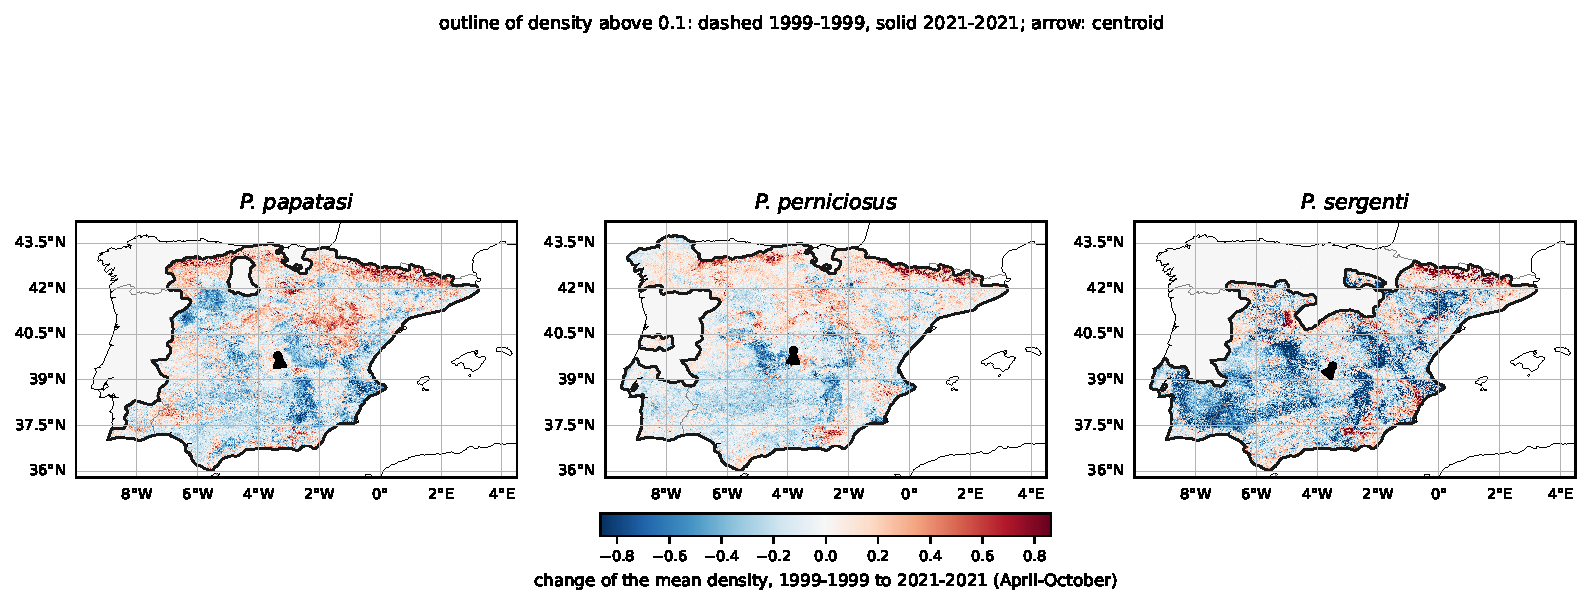
\includegraphics[width=\textwidth]{figures/fig_change_maps}
\caption{Change of the mean predicted density (April--October) from 1999--2005 to 2016--2022 per species. Lines: outline of the area above the density threshold in the early (dashed) and late period (solid). Arrow: move of the density-weighted centroid.}\label{fig:change}
\end{figure}

\begin{figure}[t]
\centering
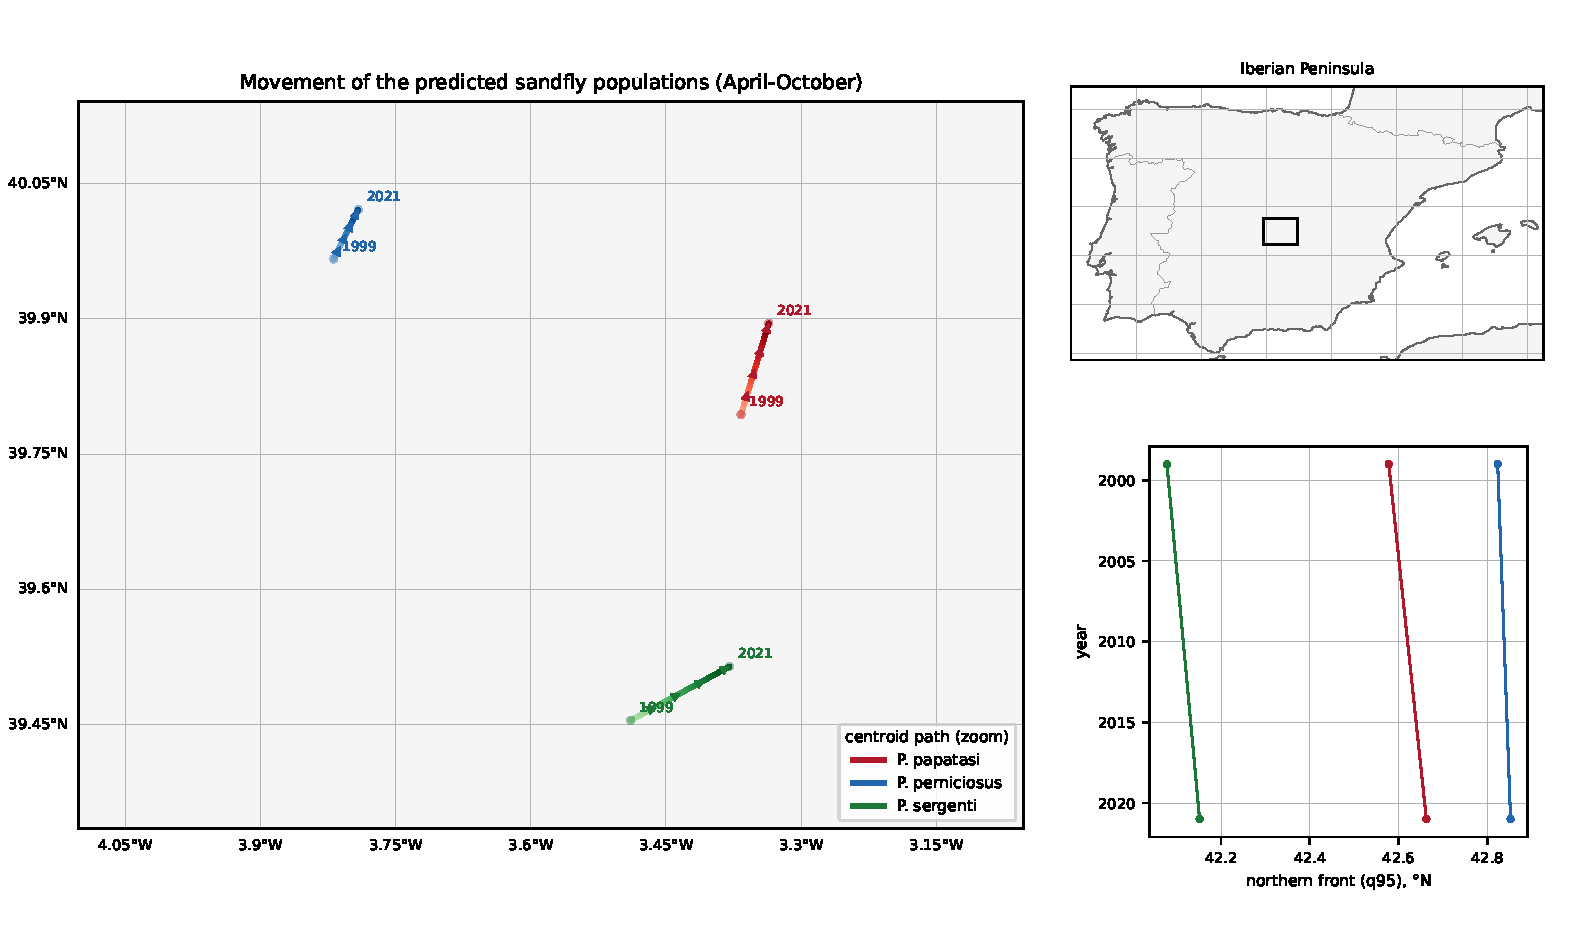
\includegraphics[width=\textwidth]{figures/fig_shift_trajectory_apr_oct}
\caption{Yearly density-weighted centroids 1999--2022 per species (light: early years, dark: late years), with the overview of the peninsula and the latitude of the northern front per year.}\label{fig:traj}
\end{figure}

\begin{table}[t]
\caption{Trends 1999--2022 (April--October): Theil--Sen slope, Mann--Kendall p-value and Pettitt change point.}\label{tab:trends}
\begin{tabular}{@{}lcccc@{}}
\toprule
Species & Centroid (km/decade) & Front (km/decade) & Occupied area (\%/decade) & Change point \\
\midrule
\spn{P.~papatasi}    & \todo{XX} & \todo{XX} & \todo{XX} & \todo{YYYY} \\
\spn{P.~perniciosus} & \todo{XX} & \todo{XX} & \todo{XX} & \todo{YYYY} \\
\spn{P.~sergenti}    & \todo{XX} & \todo{XX} & \todo{XX} & \todo{YYYY} \\
\botrule
\end{tabular}
\end{table}

\section{Discussion}\label{sec:discussion}

\todo{(1) What moves and how fast, compared with published range expansion and suitability changes \citep{Carvalho2024, Wang2025}. (2) Which predictors drive the shift (temperature against soil moisture). (3) What the shift means for One Health surveillance: the northern regions with rising vector densities are where dogs and humans are least protected and least monitored. (4) Limits: predictions, not observed migration; training data until 2022; no projection.}

\section{Conclusions}\label{sec:conclusions}

\todo{Three to four sentences.}

\backmatter

\bmhead{Acknowledgements} We thank the EDENext and VectorNet initiatives and the regional data providers and individual contributors of the FEPO training data \todo{list as in \citealp{Soheili2025}}.

\section*{Declarations}

\begin{itemize}
\item Funding: This study was funded by the European Commission through the Horizon Europe projects CLIMOS (grant 101057690, co-funded by UKRI grants 10038150 and 10039289) and PLANET4HEALTH (grant 101136652). CLIMOS is one of the six projects of the Climate Change and Health Cluster, and PLANET4HEALTH one of the five projects of the Planetary Health Cluster. The contents of this publication are the sole responsibility of the authors and do not necessarily reflect the views of the European Commission and the Health and Digital Executive Agency.
\item Competing interests: The authors declare no competing interests.
\item Data availability: \todo{FEPO output for the Iberian Peninsula, Zenodo DOI}
\item Code availability: analysis and figures, \url{https://git.ufz.de/planet4health/fepo_shift} \todo{public release}
\item Author contributions: \todo{CRediT}
\end{itemize}

\bibliography{references}

\end{document}
